

\section{Introduction}
\label{sec:intro}

A memory allocator is a key component that could significantly impact the performance and memory consumption of the corresponding applications. As an example, we evaluated \texttt{PARSEC} applications~\cite{parsec}, \texttt{Phoenix}~\cite{phoenix}, and two stress tests  \texttt{cache-thrash} and \texttt{cache-scatch} from \texttt{Hoard}~\cite{Hoard}, with multiple well-known memory allocators, such as two versions of Linux allocators (\texttt{glibc-2.28} and \texttt{glibc-2.21}), TcMalloc~\cite{tcmalloc}, \texttt{jemalloc}~\cite{jemalloc},  \texttt{Hoard}~\cite{Hoard}, and \texttt{DieHarder}~\cite{DieHarder}. Figure~\ref{fig:motivation} shows performance results of some programs, where all data in the figure is normalized to that of the Linux default allocator (\texttt{glibc-2.28}). We have the following observations: (1)~the performance difference with different allocators can be as large as $38\times$, i.e. \texttt{cache-thrash} with TcMalloc; (2)~No allocator performs consistently the best across all tested applications, indicating the importance of identifying the internal reason.
%, indicating that sometimes spending additional effort toward optimizing the application code may have a smaller  impact than simply switching to a better-suited allocator. (2)~No allocator performs consistently the best across all tested applications, indicating the importance of identifying the internal reason. 

\begin{figure}[htbp]
\centering
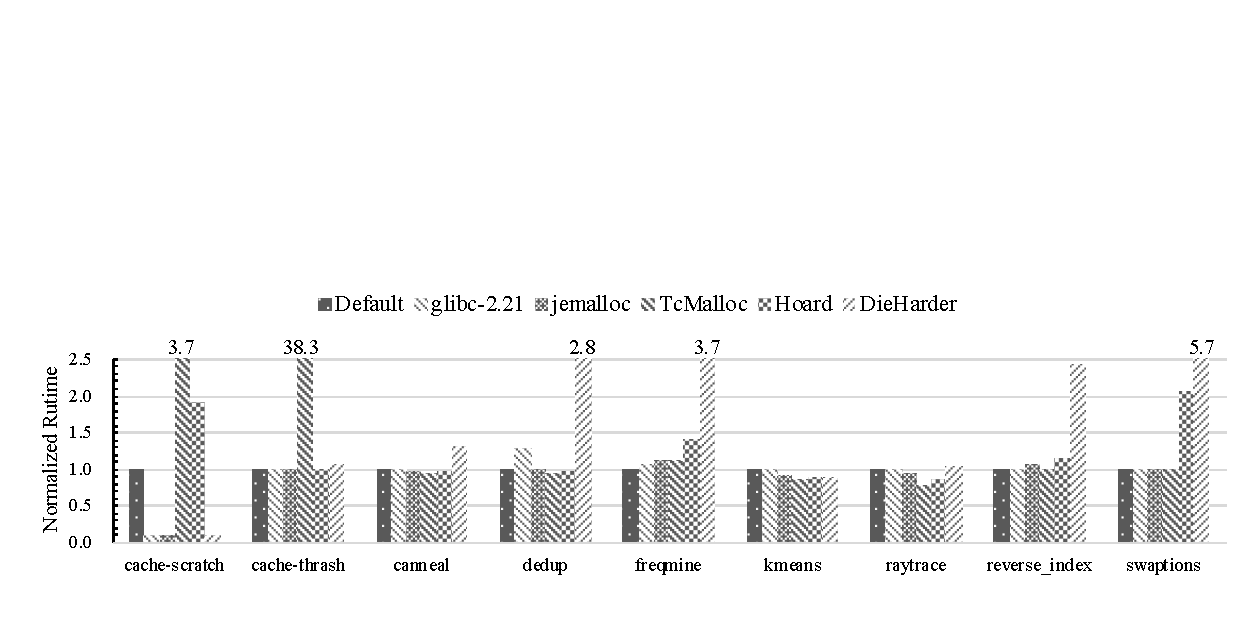
\includegraphics[width=0.98\columnwidth]{figures/motivation}
\caption{Performance Impact of Allocators\label{fig:motivation}}
\end{figure}

\begin{figure}[htbp]
\centering
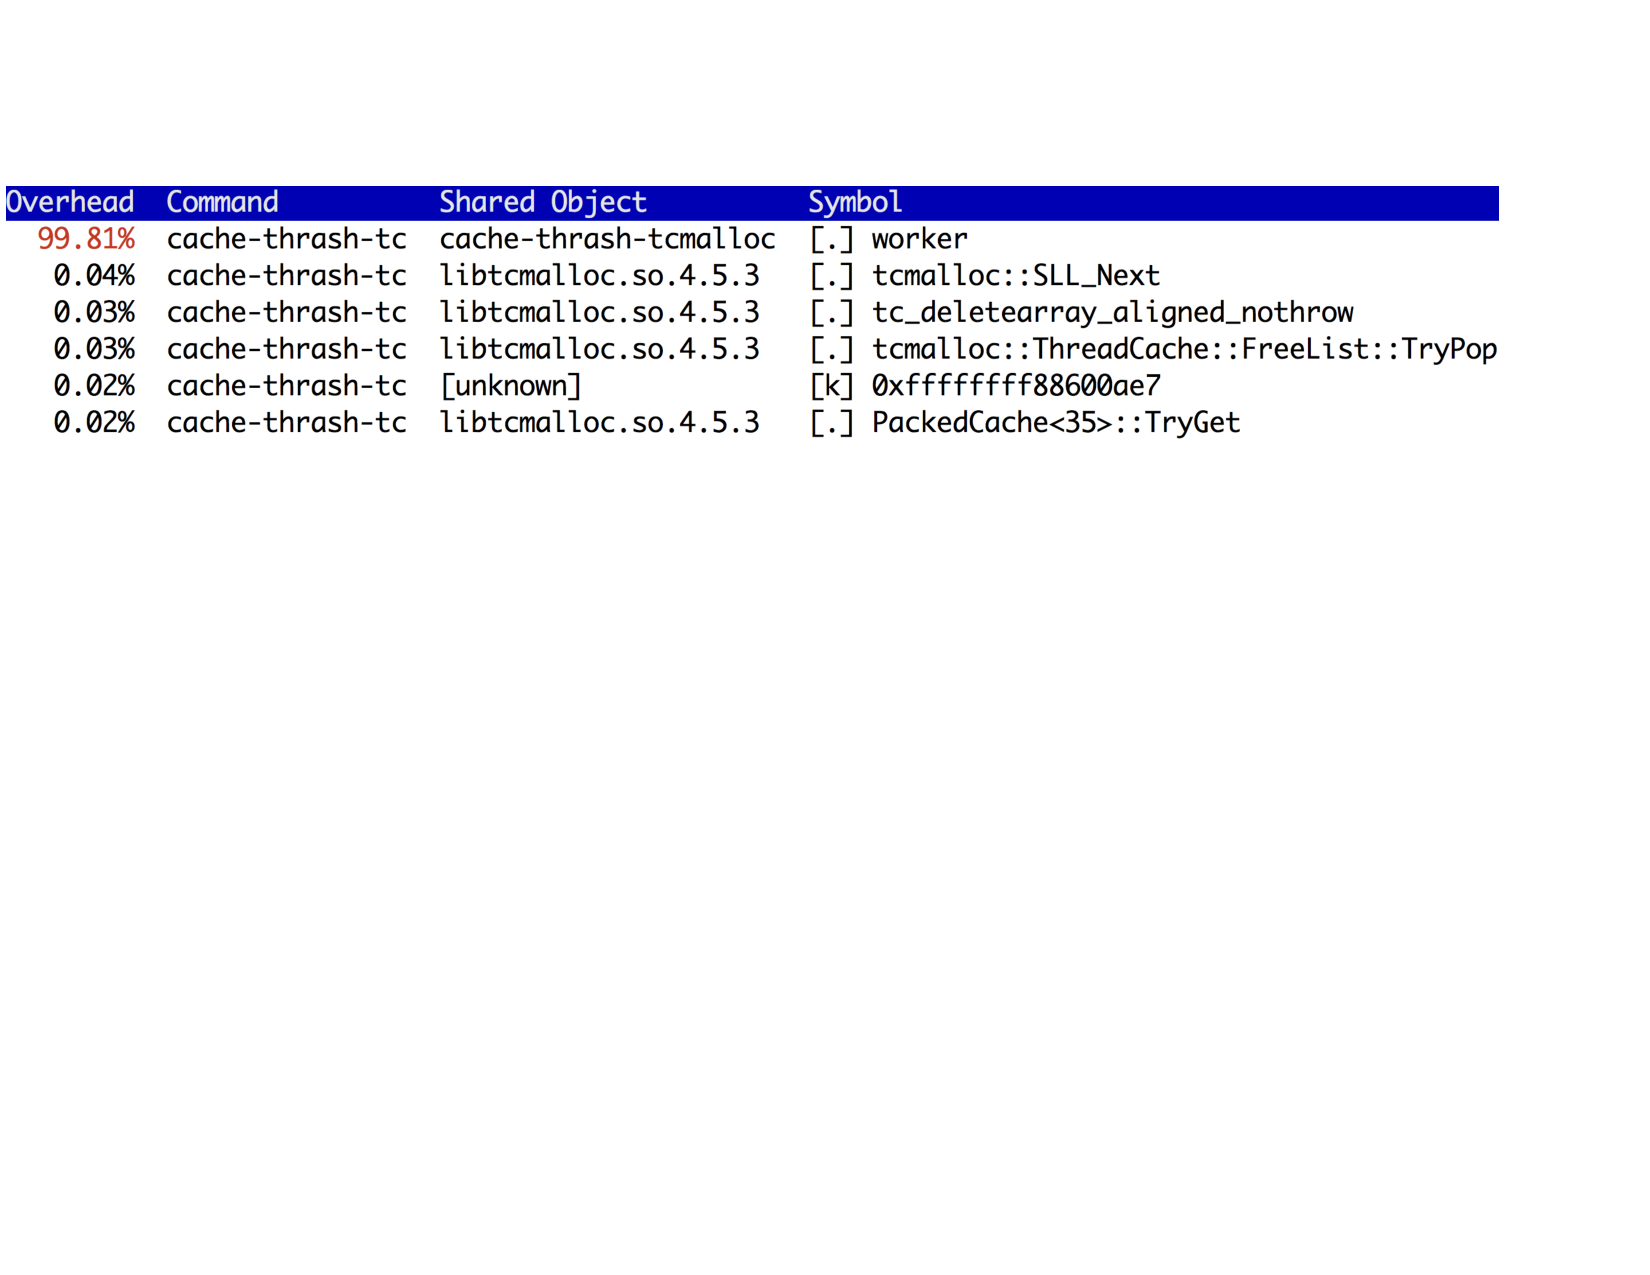
\includegraphics[width=0.95\columnwidth]{figures/perf-cache-thrash-tcmalloc}
\caption{Profiling results of \texttt{perf}. \label{fig:mot1}}
\end{figure}


Due to the obvious importance of a memory allocator, it is important to design a profiler that could answer the following questions related to an allocator. 

\begin{itemize}
\item \textbf{Q1:} \textit{Whether the allocator introduces some potential performance slowdown for this application? }
\item \textbf{Q2:} \textit{Is it possible to improve the performance and how much it can improve if switching to a well-performed allocator (e.g., TcMalloc)?}
\item \textbf{Q3:} \textit{How much memory wastes the allocator introduces?}
\item \textbf{Q4:} \textit{What are the possible design issues for a memory allocator?}
\item \textbf{Q5:} \textit{What are the reasons for memory wastes?} 
%\item What are quantitative metrics to evaluate a memory allocator? 
\end{itemize}
\vspace{0.1in}

%\todo{Jin: understand whether perf could understand the cache misses/cache invalidations based on the line number for Cache-thrash? Also, try to  whether eBPF/Ttrace or Dtrace could detect the kernel contention when running dedup with the glic-2.21? \\}

However, \textit{none of existing profilers could answer these research questions}. General-purpose performance profilers cannot identify performance issues caused by the allocator. \texttt{gprof}~\cite{DBLP:conf/sigplan/GrahamKM82} and \texttt{perf}~\cite{perf} mainly report the time accumulation of different functions, and \texttt{Coz}~\cite{Coz} presents a quantitative performance impact of improving a particular region of code. \texttt{perf}, \texttt{gprof}, and \texttt{Coz} are used to analyze the execution of \texttt{cache-thrash} with TcMalloc, since it runs around $38\times$ slower than the default Linux allocator. As shown in Figure~\ref{fig:mot1}, \texttt{perf} reports the \texttt{worker} function as the primary function to focus on. When profiling with hardware events, \texttt{perf} could even report a large number of cache misses in related lines. However, it cannot pinpoint out that the real problem is caused by the  allocator (e.g., false sharing issue introduced by TcMalloc). \texttt{gprof} reports a similar result as \texttt{perf}. \texttt{Coz} reports lines 85-87 of \texttt{cache-thrash.cpp} as the major issue, and predicts that the performance can be improved up to \textbf{10\%} if these lines can be improved by 100\%. However, it 
also did not pinpoint the real reason for the big slowdown, where TcMalloc's passive false sharing issue introduces a large number of cache invalidations as discussed in Section~\ref{sec:effectiveness}. Existing allocation profilers, such as \texttt{mprof}~\cite{Zorn:1988:MAP:894814}, Mtrace~\cite{mtrace}, Mtrace++~\cite{Lee:2000:DMM:786772.787150}, TcMalloc profiler~\cite{tcmalloc-profiler}, or CLR profiler~\cite{lupasc2014dynamic}, mainly focus on how an application uses the memory, but not memory wastes caused by an allocator. For instance, \texttt{mprof} attributes memory allocations to different allocation sites, reports memory leaks, and shows the memory usage of functions~\cite{Zorn:1988:MAP:894814}. The TcMalloc profiler reports heap usage of different allocation sites, and locates potential memory leaks~\cite{tcmalloc-profiler}. That is, these allocation profilers cannot report memory wastes caused by an allocator, which can be as big as the total memory consumption of applications. For instance, the default Linux allocator introduces 108\% memory wastes due to memory blowup for \texttt{dedup} application. 
%They cannot report performance issues caused by allocators. 

The combination of multiple profilers also cannot answer the listed questions, due to the following reasons. \textit{First}, they do not collect allocator-specific data. For instance, although \texttt{perf} is able to report the number of cache misses, it is impossible to know how many of them are actually caused by the allocator. Without that information, it is unable to determine whether some performance issues are originating from the allocator. \textit{Second}, none of existing tools collect kernel contention that is specific to the allocator, which is another source of performance issue. For instance, the glibc-2.21 allocator slows down the performance of \texttt{dedup} by more than 35\%, which is caused by frequent \texttt{madivse} system calls that directly lead to the heavy kernel contention. \textit{Third}, none of existing profilers can answer whether switching an allocator could improve the performance for one application or not, without the performance-related parameters, such as memory management latency, application-friendliness, user-space and kernel-space contention caused by the allocator. Certainly, users could try popular memory allocators one by one,  but they never know whether another allocator could actually perform better on this application. Therefore, there is an urgent need of a new profiler that could answer all listed questions as above. 
%Third, none of existing profilers report the application friendliness of an allocator, such as false sharing issues caused by the allocator.


%\todo{Without that information only of the allocator, the user cannot know how the allocator affects their applications. If there is a tool quantitatively revealing the performance and memory effects made by the allocator, users will absolutely know whether it is necessary to switch their allocator or not, which could save a lot of time from the wrong side. Also, those tools could not help allocator designers improve their works in short of detailed information about the allocator itself.}

%\todo{There are some popular performance analyzers, such as \texttt{ftrace}~\cite{ftrace} and \texttt{dtrace}~\cite{dtrace}. However, they can not answer those questions, and they even have other limitations. For example, to get different information from \texttt{ftrace}, users have to manually switch the current tracer and run their programs multiple times. \texttt{dtrace} requires root privileges to get into the kernel. Both of those limitations create huge inconvenience for normal users and allocator designers.}
%In addition, those general-purpose profilers cannot identify the performance issues of a memory allocator, 

This paper presents such an allocator profiler--\MP{}--that helps answer these questions. \MP{} will benefit both normal users and allocator designers, since normal users could benefit from answers of the first three questions, and allocator designers could utilize it to pinpoint design issues latent inside an allocator (related to \textbf{Q4} and \textbf{Q5}). This profiler aims to profile different allocators without changing the allocator and the application code. The basic idea of the profiler is further discussed as follows. 
%, so that there is no need to reinvent the wheel for allocator designers, when they design a new allocator or improve an existing allocator. 

In order to answer the question \textbf{Q1}, it is necessary to understand how an allocator could actually affect the performance of applications. Since an allocator will manage memory allocations and deallocations from applications, it can affect applications in two ways: first, the performance of memory management operations will affect the performance of applications, which can be further caused by many factors, such as implementation complexity (e.g., number of instructions), user-space contention, and kernel-space contention. Second, whether an allocator is tapping well with memory usage and access pattern of a particular application, called ``\textit{application friendliness}'' in the remainder of this paper. That is, even a fast allocator could significantly degrade the performance, if it is not tapping well with memory usage pattern of the application. For the previous example (e.g., \texttt{cache-thrash}), the  high-performant TcMalloc actually slows down by $38\times$ (as shown in Figure~\ref{fig:motivation}) due to its friendliness issue. \MP{} will report application-friendliness of an allocator, including cache utilization rate, page utilization rate, passive/active false sharing, and cache invalidation rate (outside allocations/deallocations). \MP{}  proposes the combination of time-stamp and hardware performance counters to perform the profiling, as further described in Section~\ref{sec:background}. 
%in order to reduce the performance overhead. For instance, to collect cache utilization rate, \MP{} tracks used bytes of every cache line, and then updates the overall cache utilization rate upon every sampled access. Overall, these parameters will help users to understand the performance degradation on a specific application. For the previous example, \MP{} reports that the passive false sharing is the direct reason for TcMalloc's low performance on \texttt{cache-trash} application.


% It is straightforward to collect the cycles of memory management operations during the execution. Then we propose to replace the collected cycles with those of a target allocator in order to predict the possible performance impact after switching to the target allocator, which helps 
% \todo{users identify how the allocator could affect application performance, and decide whether they should switch their allocator or not.}

It is difficult to answer the question \textbf{Q2}, but will be very useful for normal programmers: they do not need to search for a better allocator, if the profiler could predict that there is no need to do so. \MP{}'s prediction will be based on the above discussion: if the current allocator has a good performance, and the allocator is very application-friendly. It is impossible to accurately predict the performance impact caused by application-friendliness, such as false sharing effect, cache utilization, or page utilization. Instead, \MP{} will give a qualitative prediction on this: users don't need to change the allocator, if all parameters of application-friendliness are normal. \MP{} is able to predict the performance impact caused by the allocator's performance, by replacing the collected cycles with those of a target allocator.   However, a naive solution may not work well due to the following reasons. First, different types of allocations have substantially different performance, as shown in Table~\ref{tbl:metrics}, such as allocations of small and big objects, serial and parallel phase, new and reused allocations, allocations and deallocations. Second, the target allocator may has a different threshold for small and big objects from the current allocator. The third issue can be caused by the parallelization of multithreaded applications. \MP{} solves all of these issues as discussed in Section~\ref{sec:predict}.

The question \textbf{Q3} is related to memory wastes caused by the allocator. The straightforward method is to intercept memory-related system calls (e.g., \texttt{mmap} and \texttt{sbrk}) inside memory operations to collect the total memory consumption, and then subtract it by consumption of applications. However, virtual memory is different from physical memory, since physical pages are typically allocated on demand inside the OS. In addition, the allocator may return physical pages to the OS via \texttt{madvise} or \texttt{munmap}. Instead, \MP{} proposes a page-based mechanism to track memory consumption, where a page is treated as ``allocated'' if some objects in this page have been allocated to the application. It further tracks \texttt{madvise} and \texttt{munmap} to update memory consumption timely. 

To answer the question \textbf{Q4}, \MP{} identifies all important factors that may affect the performance of memory management operations: the complexity of the implementation, efficiency management operation, user space contention, and kernel space contention. For each operation, \MP{} utilizes the averaged number of instructions and other hardware events to evaluate the implementation complexity and efficiency, measures the number of lock acquisitions and lock contention rate, and employs the average time of memory related system calls to evaluate kernel contention. Overall, \MP{} proposes to utilize hardware Performance Monitoring Units (PMUs) to collect the number of instructions and hardware events, and intercepts synchronizations and memory related system calls in order to identify user and kernel space contention. 
%we should understand the reasons of slow memory management operations. B,  The second reason can be caused by hardware events of the algorithm design, such as cache misses. The third reason can be caused by user space contention, which could be evaluated via lock acquisitions and lock contention inside each memory management operation. The fourth reason is due to kernel contention, which could be caused by memory-related system calls. All of these reasons have been observed in different allocators, as further discussed in Section~\ref{sec: benifitdesigners}.  
%and it also introduces multiple cache misses for each free operation. 
%Both DieHarder and Hoard has a high number of lock acquisitions and high contention rate for some applications, and Glibc-2.21 has high kernel contention for \texttt{dedup}. 

For Question \textbf{Q5}, \MP{} reports different types of memory wastes introduced by an allocator. Although it is straightforward to measure internal fragmentation, but not for memory blowup and external fragmentation. Memory blowup occurs when memory deallocations from one thread cannot be utilized to satisfy subsequent memory requests from other threads~\cite{Hoard}, due to the employment of per-thread heaps. However, this definition cannot be utilized directly to collect the total memory blowup, as it does not specify how to update it upon successive deallocations and re-allocations. \MP{} measures memory blowup with a key observation: \textit{the total size of freed objects represents the upper bound of memory blowup for a size class}. Then the memory blowup can be measured by subtracting the total size with the size of recently-freed objects. After computing the memory blowup, \MP{} is able to compute the external fragmentation afterwards, using the total memory consumption. 



 %\textit{The novelty (and challenge) of \MP{} lies in its decision of what to profile and how to profile precisely and efficiently}, as described in the following. First, \MP{} profiles the performance impact of memory management operations, which will directly affect the performance of running an application. It is straightforward to utilize the time (cycles) of each allocation and deallocation as the metrics, but there exist multiple issues. 
 
 %The second issue is that the runtime itself cannot tell the underlying reason for the performance issue. Instead, \MP{} differentiates the data based on allocation types, such as small/large allocation, new/re-used allocation, which helps identify the real issue inside the allocator. In addition, \MP{} proposes to utilize hardware Performance Monitor Units (PMUs) to collect hardware related events (instructions, cache misses, or page faults), and intercept synchronizations and memory-related system calls to obtain user-space and kernel contention, helping understand the particular design issue inside. For instance, glibc-2.21 invokes a large number of \texttt{madvise} system calls for the \texttt{dedup} application~\cite{madvise}, where the system call overhead and unnecessary page faults are the major reason of 28\% slowdown. 
%\MP{} is able to report such issues by intercepting memory-related system calls. 

Overall, \MP{} profiles multiple important aspects of memory allocators, such as performance, memory, scalability, and application-friendliness. Based on our extensive evaluation, \MP{} successfully identifies multiple known and \textbf{unknown} design issues inside popular allocators, as further described in Section~\ref{sec:effectiveness}. Due to its careful design, \MP{} only imposes 35\% performance overhead on average. This efficient design reduces \MP{}'s interference to the original execution. \MP{} does not need the change of the allocator, the application, and the underlying OS, which will be convenient for its employment. 

%\todo{one way to highlight the contribution is to emphasize on the **complex** considerations of designing good allocators and the challenges to identify design problems. We want to let the reviewer know that it's difficult to do. }

\subsection*{Contribution}

Overall, this paper makes the following contributions. 

\begin{itemize}
\item \MP{} proposes a systematic approach to evaluate and profile different memory allocators, without changing the code of allocators or applications. More specifically, \MP{} proposes the combination of function interception (based on common APIs) and PMU-based sampling to perform the profiling.

%It proposes the first general profiler--\MP{}--to profile different memory allocators, without the need of the change of the allocator and the underlying OS, if an allocator utilizes the standard synchronization and system calls.  

\item \MP{} presents relevant factors that may impact the performance and memory consumption of applications, and provides some metrics for efficient allocators, which could benefit future allocator designers. 
%important reasons that may impact  of an allocator that will significantly impact the performance and memory overhead of an allocator, with the assistance of PMUs, time-stamp counters, and simple counters together. 

\item \MP{} performs an experimental evaluation to quantitatively measure the performance, memory wastes, cache/page utilization rate, and passive/active false sharing of multiple widely-used allocators. 
%, multiple practical methods to profile some metrics precisely and efficiently for the first time, such as memory blowup, . 
%profile cache/page utilization rate, memory blowup, active/passive false sharing, and kernel contention for the first time.
%, and attributes the data to each allocation and deallocation, helps discover designing issues that cannot be discovered with general profilers.  
%\item \MP{} proposes a practical method to predict the performance impact of the current allocator, which allows normal users to 
\item This paper performs extensive experimentation to confirm \MP{}'s effectiveness and low overhead. These experiments also uncover multiple known and unknown design issues in widely-used allocators.  

\end{itemize} 

\begin{comment}

%\todo{What is new in this tool? Whether it could provide some information that is not available in an existing allocator.}

\begin{itemize}
\item It will quantify application-friendliness, which is not available in existing work, and which helps users to decide which allocator should be used for a specific application. 
\item It will provide the memory usage (overhead) information, such as internal fragmentation, and objects that are not freed but yet which remain unused. 
\item It will provide some information that only exists across multiple profilers, for instance, the average number of instructions of each allocation and deallocation, the average time spent within each allocation and deallocation (PMU sampling will be placed outside of the time span, thus not avoiding an erroneous measurement of how long this allocation and deallocation request has been sampled), whether there are some contentions during allocation (user space and kernel space), how many lock acquisitions.  
\end{itemize}
 	
\end{comment}

\subsection*{Outline}

The remained of this paper is organized as follows. Section~\ref{sec:background} discusses the background of memory allocators, and the basic idea of \MP{}. Then Section~\ref{sec:implementation} presents the detailed implementation. After that, Section~\ref{sec:evaluation} shows experimental results on different allocators using \MP{}, and Section~\ref{sec:limitation} discusses a potential limitation. In the end, Section~\ref{sec:relatedwork} discusses related work in this field, and Section~\ref{sec:conclusion} concludes this paper.